\documentclass[a4paper,12pt]{book}
\usepackage[table]{xcolor}
\usepackage{amsmath}
\usepackage{amssymb}
\usepackage[utf8]{inputenc}
\usepackage[T1]{fontenc}
\usepackage[francais]{babel}
\usepackage{graphicx}
\usepackage[colorlinks]{hyperref}
\usepackage{makeidx}
\usepackage{lipsum} 
\usepackage{a4wide}
\usepackage{svg}
\usepackage{mathrsfs}

\makeatletter

\title{Les notes de Rancune: \\Electronique Analogique}
\author{Rancune}
\date{\today}

\makeindex

\begin{document}

\maketitle

\frontmatter

\tableofcontents    

\mainmatter

\chapter*{Introduction}
\addcontentsline{toc}{part}{Introduction}


\part{ Les lois de base }

\chapter{Les grandeurs électriques}

\section{La charge électrique}

\begin{tabular}{ll}
\textbf{Notation usuelle~:} & $Q$, $q$ \\
\textbf{Unité~:} & Coulomb (C) \\
\textbf{Unité SI~:} & $A \cdot s $ \\
\textbf{Nature~:} & Grandeur scalaire \\
\end{tabular} 

\subsection*{Définition}

\index{charge!charge electrique@charge électrique}

Tout comme la masse pour les interactions gravitationnelles, la \textbf{charge électrique} est une propriété fondamentale de la matière qui lui permet d'intéragir par le biais de champs électromagnétiques. \\ 

Il existe deux types de charges électriques : les charges positives ($+$) et les charges négatives ($-$). Deux charges de même signe se repoussent, deux charges de signes différents s'attirent.\\

On appelle \textbf{porteur de charge} une particule ou un corps portant une charge non nulle. Bien qu'on pense en général aux électrons lorsqu'on parle de courant électrique, ceux-ci ne sont pas les seuls porteurs de charges. Les protons et les ions (anions et cations), par exemple, en sont également. 

\index{charge!porteur de charge}

\subsection*{ Quantification de la charge~: }

\textbf{La charge électrique est quantifiée} : elle est un multiple entier de la \textbf{charge élémentaire} $e$, qui correspond à la charge d'un électron.
\index{electron@électron}
\index{charge!charge elementaire@charge élémentaire}
\index{charge!quantification de la charge}

\begin{equation}
	e \approx 1,602.10^{-19} C
\end{equation}

Néanmoins, on la considère en général en électronique comme une grandeur continue. Ceci a pour conséquence d'introduire dans les calculs un bruit particulier, appelé "bruit de grenaille".
\index{bruit!bruit de grenaille}
\index{grenaille!bruit de grenaille}

\subsection*{ Conservation de la charge~: }

\textbf{La charge électrique est une grandeur conservative}~: la charge d'un système isolé est invariante. La charge electrique ne peut donc être qu'échangée avec un autre système, mais ni créée, ni annihilée.
\index{charge!conservation de la charge}

\section{Le potentiel}

\begin{tabular}{ll}
\textbf{Notation usuelle~:} & V \\
\textbf{Unité~:} & Volt (V)\\
\textbf{Unité SI~:} & ${kg} \cdot m^2 \cdot {s}^{-3} \cdot A^{-1}$ \\
\textbf{Nature~:} & Grandeur scalaire \\ 
\end{tabular}

\subsection*{Définition}

En tout point de l'espace est défini un \keyword{potentiel}. Cette valeur scalaire correspond à l'énergie potentielle électrostatique que posséderait une charge électrique unitaire située en ce point. \\ 

Les points possédant une même valeur de potentiel sont désignés sous le nom d'\textbf{équipotentielle}.\index{equipotentielle@équipotentielle}

\subsection*{La terre}

Le \textbf{potentiel zéro} est par convention le potentiel de la \textbf{terre}, obtenu en plantant un piquet conducteur en terre. On le suppose en général égal en tout lieu mais c'est une approximation. \\

Cet équipotentiel zéro est noté avec le terme anglais "Ground" (ou GND en abbrégé) dans les circuits. On le représente avec le symbole suivant~:

\begin{figure}[!h]
\centering
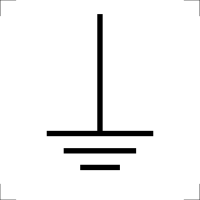
\includegraphics{part01/chap01/ground.png}
	\caption{Symbole représentant la terre \\ norme IEC 60417 }
\end{figure}

\index{terre}
\index{ground}

\section{La tension}

\begin{tabular}{ll}
\textbf{Notation usuelle~:} & $U$, $u$, $U_{AB}$ \\
\textbf{Unité~:} & Volt (V) \\
\textbf{Unité SI~:} & ${kg} \cdot m^2 \cdot {s}^{-3} \cdot A^{-1}$ \\
\textbf{Nature~:} & Grandeur scalaire \\
\end{tabular} 

\subsection*{Définition}

Une \keyword{tension} $U_{AB}$ est la circulation du champs électrique le long d'un circuit $\mathscr{C}$ entre les points $A$ et $B$~:

\begin{equation}
	U_{AB} = \int_{\mathscr{C}_{A}}^{\mathscr{C}_B}\vec{E}\,dl
\end{equation}

Cependant, cette définition est trop détaillée pour l'électronique. En effet, si l'on suppose que le temps de propagation des ondes électromagétiques est négligeable (hypothèse du régime stationnaire), la tension est alors égale à la "\textbf{différence de potentiel}" entre les deux extrémités du circuit.

\begin{equation}
	U_{AB} = V_A - V_B
\end{equation}

\index{potentiel!difference de potentiel@différence de potentiel}

\subsection*{Représentation graphique: }

\begin{minipage}{7cm}
\begin{center}
\includesvg{part01/chap01/tension}
\end{center}
\end{minipage}
\hspace{1cm}
\begin{minipage}{7cm}
Une tension est représentée par une flêche. Son sens est important car une tension est une \underline{grandeur signée}. 
\end{minipage}\\

\subsection*{Mesure d'une tension}

En électronique, une tension se mesure toujours \emph{entre deux points}, à l'aide d'un voltmètre (ou d'un oscilloscope si on veut en voir les variations temporelles). \\


\begin{minipage}{7cm}
\begin{center}
\includesvg{part01/chap01/mesure_tension}
\end{center}
\end{minipage}
\hspace{1cm}
\begin{minipage}{7cm} 
	Le voltmètre se connecte en parallèle de la tension à mesurer. 
\end{minipage}\\

\section{Le courant}

\begin{tabular}{ll}
\textbf{Notation usuelle~:} & $I$, $i$ \\
\textbf{Unité~:} & Ampère (A) \\
\textbf{Unité SI~:} & $A$ \\
\textbf{Nature~:} & Grandeur scalaire \\
\end{tabular} 

\subsection*{Définition}

Un \textbf{courant} est un mouvement d'ensemble de porteurs de charges électriques au sein d'un matériau conducteur. Ces porteurs de charge sont dans le cas le plus courant des électrons, mais cela peut également être des ions positifs ou négatifs (Par exemple dans le cas des electrolytes) ou encore n'importe quel corps portant une charge non nulle. 

\index{courant!courant électrique}

\subsection*{ Représentation graphique: }

\begin{minipage}{7cm}
	\includesvg{part01/chap01/courant} 
\end{minipage}
\hspace{1cm}
\begin{minipage}{7cm}
	Le courant électrique est généralement représenté par une flêche située sur le circuit. Son sens est important car un courant est une \underline{grandeur signée}. 
\end{minipage}\\

\subsection*{Mesure d'un courant électrique }

En pratique, un courant se mesure généralement à l'aide d'un ampèremètre. \\ 

\begin{minipage}{7cm}
\begin{center}
\includesvg{part01/chap01/mesure_courant}
\end{center}
\end{minipage}
\hspace{1cm}
\begin{minipage}{7cm} 
	L'ampèremètre se connecte en série sur le circuit dans lequel on veut mesurer un courant. 
\end{minipage}\\

\index{courant!mesure du courant}
\index{amperemetre@ampèremètre}

\subsection*{ Sens conventionnel du courant: }

Par convention, le courant sort du générateur électrique par la borne positive et y revient par la borne négative. C'est ce que l'on appelle le \textbf{sens conventionnel du courant}. \\
\index{courant!sens conventionnel du courant}
\index{conventionnel!sens conventionnel du courant}

On ne raisonne jamais en électronique en utilisant le sens réel des porteurs de charges, car celui-ci sera différent s'il s'agit d'électrons (qui circulent du pôle négatif vers le pôle positif du générateur) ou de cations (qui circulent en sens inverse). Cela n'a aucune importance et ne ferait que complexifier inutilement les raisonnements. Dans la suite de ce document, et plus largement dans l'intégralité des ouvrages lus par votre serviteur, c'est toujours le sens conventionnel qui est utilisé.

\subsection*{Intensité du courant}

L'\keyword{intensité} du courant électrique (parfois appelée "\keyword*{ampérage}" ou "\keyword*{courant}") correspond au débit de charges électriques à travers une surface donnée (le plus souvent la section d'un fil électrique)~: 

\begin{equation}
	i(t) = \dfrac{dq}{dt} 
\end{equation}

avec~: \\
\begin{itemize}
	\item[$\bullet$] $i$ : l'intensité du courant
	\item[$\bullet$] $q$ : la charge électrique
	\item[$\bullet$] $t$ : le temps.
\end{itemize}

\section{L'énergie électrique}

\begin{tabular}{ll}
\textbf{Notation usuelle~:} & $E$ \\
\textbf{Unité~:} & Joule (J) \\
	\textbf{Unité SI~:} & $kg \cdot m^2 \cdot s^{-2}$ \\
\textbf{Nature~:} & Grandeur scalaire \\
\end{tabular} 

\subsection*{Définition}

\textbf{Parler d'énergie électrique est au sens strict un abus de langage}. Ce n'est pas une véritable forme d'énergie comme peuvent l'être l'énergie cinétique ou l'énergie potentielle. Il s'agit plutôt d'un vecteur énergétique, c'est à dire un moyen de transférer de l'énergie entre deux systèmes : l'électricité requiert et transporte de l'énergie.\\
\index{energie@énergie}

L'énergie électrique est définie de la façon suivante~:

\begin{equation}
	E = q \cdot U
\end{equation}

avec~:\\
\begin{itemize}
	\item[$\bullet$] $E$ la quantité d'énergie en joules
	\item[$\bullet$] $q$ la charge électrique en coulombs
	\item[$\bullet$] $U$ la tension électrique en volts
\end{itemize}

\subsection*{Autre unité de mesure}

Le joule étant une unité de mesure assez petite pour les besoins des électriciens, une autre unité est souvent utilisée~: le kiloWattheure (kWh). 
\index{kiloWattheure}

$$ 1\:kWh = 10^3 \cdot 3600\:J = 3.6\:MJ $$


\subsection*{Lien avec la puissance}

si $I$ est le courant, la quantité de charges qui circulent pendant un temps $\Delta t$ est~: 

$$q = I \cdot \Delta t$$

(On suppose le courant constant pendant l'intervalle de temps).\\

La quantitée d'énergie échangée $E$ pendant $\Delta t$ est donc~:

$$ E = q \cdot U = I \cdot \Delta t \cdot U = U \cdot I \cdot \Delta t $$

Ce qui amène à~: \\
\begin{equation}
E = P \cdot \Delta t 
\end{equation}

avec $P$ la puissance électrique.

\section{La puissance électrique}

\begin{tabular}{ll}
\textbf{Notation usuelle~:} & $P$ \\
\textbf{Unité~:} & Watt (W) \\
	\textbf{Unité SI~:} & $kg \cdot m^2 \cdot s^{-3}$ \\
\textbf{Nature~:} & Grandeur scalaire \\
\end{tabular} 

\subsection*{Définition}

\textbf{La puissance électrique}\index{puissance!puissance electrique@puissance électrique} est un taux d'énergie transférée par un circuit électrique par unité de temps. La puissance est donc reliée à l'énergie échangée par la relation~:

\begin{equation}
	P = \dfrac{E}{\Delta t}
\end{equation}

Ce qui nous permet également de l'exprimer en fonction de la tension et du courant :

\begin{equation}
	P = U \cdot I
\end{equation}

Pour un générateur, cette quantité est négative (le générateur fournit de l'énergie). Pour une charge, cette quantité est positive.


\chapter{Les circuits électriques}

\section{Circuit électrique}

\index{circuit!circuit électrique@circuit électrique}
\index{potentiel!difference de potentiel@différence de potentiel}
\index{stationnaire!hypothèse du régime stationnaire}
\index{hypothèse!hypothèse du régime stationnaire}
\index{conducteur!conducteur parfait}

Si l'on a un regard de physicien sur un schéma électronique, il devient très difficile de réfléchir sur un circuit tant les choses sont complexes. Les ondes électromagnétiques se propagent dans les conducteurs selon des lois difficiles à appréhender, et il se passe bien des choses entre et dans chaque composant. L'électronique repose donc sur quelques hypothèses de simplification nous permettant de raisonner simplement.  

La première de ces hypothèses est l'\textbf{hypothèse du régime stationnaire}. Celle-ci implique que la propagation des ondes électromagnétiques est supposée terminée, et que nous pouvons négliger les effets qui en découlent. Ceci à deux conséquences : 

\begin{itemize}
\item \textbf{La tension est assimilée à la différence de potentiel} \\
\item \textbf{Dans un conducteur parfait (de résistance nulle), la différence de potentiel est nulle.}
\end{itemize}

\index{blocs!blocs fonctionnels}
\index{lumped!lumped elements}
\index{elements!lumped elements}
La seconde hypothèse importante est celle des \textbf{blocs fonctionnels} ("lumped elements" en anglais)~: ceci consiste à considérer que l'on peut représenter un circuit comme un ensemble de blocs simples (résistance, capacité, inductance, etc.) reliés entre eux par un réseau de fils parfaitement conducteurs.

Sauf mention contraire (Par exemple quand nous nous intéresserons aux radiofréquences pour lesquelles on ne peut plus négliger la propagation des ondes), nous supposerons toujours ces hypothèses valides.

\pagebreak
\section{Les dipôles}

\index{dipole@dipôle}
Un \textbf{dipôle}, comme son nom l'indique, est un composant dôté de deux bornes. On peut citer comme exemple de dipôle les résistances, les condensateurs, les bobines, les diodes, etc. Le problème est alors que les tensions, tout comme les intensités, sont des grandeurs signées. Afin de pouvoir caractériser un composant, il nous faut donc se mettre d'accord sur la manière de les choisir.

\subsection*{Convention recepteur}

\index{recepteur@récepteur}
\index{convention!convention recepteur@convention récepteur}
\index{recepteur@récepteur!convention recepteur@convention récepteur}
\index{dipole@dipôle!dipole recepteur@dipôle récepteur}
Pour les dipôles récepteurs, c'est à dire les dipôles prenant de l'énergie au circuit, la convention adoptée est la \textbf{convention récepteur}. Elle consiste à placer les flêches de tension et de courant dans des sens opposés. 

\begin{figure}[!h]
\centering
\includesvg{part01/chap02/convention_recepteur}
\caption{Dipôle en convention récepteur}
\end{figure}

Les différentes lois que nous allons écrire pour les composants (la loi d'Ohm par exemple) seront exprimées selon cette convention.

\subsection*{Convention générateur}

\index{generateur@générateur}
\index{convention!convention generateur@convention générateur}
\index{generateur@générateur!convention generateur@convention générateur}
\index{dipole@dipôle!dipole generateur@dipôle générateur}
Pour les dipôles générateurs, c'est à dire les dipôles fournissant de l'énergie au circuit, la convention adoptée est la \textbf{convention générateur}. Elle consiste à placer les flêches de tension et de courant dans le même sens. 

\begin{figure}[!h]
\centering
\includesvg{part01/chap02/convention_generateur}
\caption{Dipôle en convention générateur}
\end{figure}

Les différentes lois que nous allons écrire pour les générateurs (batteries, piles, sources de signal, etc.) seront exprimées selon cette convention.

\subsection*{Signe de la puissance électrique}

\index{puissance!puissance electrique@puissance électrique}
\index{puissance!convention generateur@convention générateur}
\index{puissance!convention recepteur@convention récepteur}
\index{puissance!signe}
Dans l'expression du calcul de la puissance, $P=U \cdot I$, le signe du résultat va donc dépendre de la convention utilisée.

\begin{table}[!h]
\begin{center}
\bgroup
\def\arraystretch{1.5}%  1 is the default, change whatever you need
\rowcolors{2}{blue!30}{blue!10}
\begin{tabular}{|c|c|c|}
	\hline
	& \textbf{Convention Récepteur} & \textbf{Convention Générateur} \\
	\hline
	Récepteur physique  & $P<0$ & $P>0$ \\
	\hline
	Générateur physique & $P>0$ & $P<0$ \\
	\hline
\end{tabular}
\egroup
\end{center}
	\caption{ Signe de la puissance }
\end{table}

\section{Lois de Kirchhoff}
\index{kirchhoff}
\index{kirchhoff!lois de Kirchhoff}
\textbf{Les lois de Kirchhoff} expriment la conservation de l'énergie et de la charge dans un circuit électrique. Au nombre de deux (la loi des noeuds et la loi des mailles), elles permettent de déterminer les valeurs courants et les tensions dans le circuit.

\subsection*{Loi des noeuds}
\index{kirchhoff!loi des noeuds}
\index{noeud!loi des noeuds}
\index{courant!loi des noeuds}
\index{noeud}
\vspace{0.5cm}
\begin{minipage}{3cm}
\begin{center}
\includesvg{part01/chap02/loi_des_noeuds}
\end{center}
\end{minipage}
\hspace{1cm}
\begin{minipage}{10cm} 
\textbf{La somme des intensités des courants qui entrent par un noeud est égale à la somme des intensités des courants qui sortent du même noeud.} \\
	$$ I_2 + I_3 = I_1 + I_4 $$
\end{minipage}\\

\smallskip
Cette loi découle directement de la conservation de la charge électrique, en tenant compte du fait qu'en régime stationnaire, ces charges ne peuvent pas s'accumuler à un endroit quelconque du circuit. Pour un noeud, cela veut donc dire que la quantité de charge entrante est égale à la quantité de charges sortantes.\\

\subsection*{Loi des mailles}
\index{kirchhoff!loi des mailles}
\index{tension!loi des mailles}
\index{maille!loi des mailles}
\index{maille}
\vspace{0.5cm}
\begin{minipage}{3cm}
\begin{center}
\includesvg{part01/chap02/loi_des_mailles}
\end{center}
\end{minipage}
\hspace{1cm}
\begin{minipage}{10cm} 
\textbf{Dans une maille quelconque d'un circuit, la somme des différences de potentiel le long de la maille est nulle.} \\

\hspace{1cm}
\begin{minipage}{8cm} 
Exemple~:
\begin{center}
$  U_1 - U_2 - U_3 - U_4 + U_6 = 0$ (Maille 1) 
\end{center}
Ou pour la maille passant par $U_5$~:
\begin{center}
$ U_1 - U_2 -U_3 - U_5 + U_6 = 0 $
	\end{center}
\end{minipage}\\
\end{minipage}\\

\smallskip
Cette loi est valable dans l'approximation des régimes stationnaires, et à condition que les variations de flux magnétique à travers la maille soient négligeables.

\section{Théorème de Millman}

\textbf{Le théorème de Millman} est une variante de la loi des noeuds, écrite sous la forme de potentiels. Il s'énonce de la façon suivante~:\\

\index{millman!theoreme de millman@théorème de Millman}
\index{noeud!theoreme de millman@théorème de Millman}
\index{potentiel!theoreme de millman@théorème de Millman}
\vspace{0.5cm}
\begin{minipage}{5cm}
\begin{center}
\includesvg{part01/chap02/millman}
\end{center}
\end{minipage}
\hspace{1cm}
\begin{minipage}{10cm}

	\textbf{Pour un noeud $M$, auquel sont connectées des branches contenant des résistances $R_i$ reliées à des potentiels $V_i$, le potentiel $V_M$ s'écrit~:}

\begin{equation}
	V_M = \dfrac{\displaystyle\sum_{i}\dfrac{V_i}{R_i}}{\displaystyle\sum_{i} \dfrac{1}{R_i} }
\end{equation}

\end{minipage}\\

\smallskip
Ce théorème peut également s'écrire avec des tensions (différences de potentiel).


%\input{ résistance.tex }
%\input{ capacité.tex }
%\input{ inductance.tex }

%\part{ Les composants Linéaires }

%\input{ resistor.tex }
%\input{ condensateur.tex }
%\input{ bobine.tex}

%\part{ Les semi-conducteurs }

%\input{ diode.tex }
%\input{ bjt.tex }
%\input{ fet.tex }

%\part{ Analyse harmonique }

% Les annexes

\part{Annexes}
\appendix

\chapter{Les unités}

\section{Les unités S.I.}

Les septs unités du système SI sont les unités à partir desquelles on peut contruire toutes autres unités en physiques. Ces sept unités de bases sont les suivantes~:

\begin{center}
\bgroup
\def\arraystretch{1.2}%  1 is the default, change whatever you need
\rowcolors{2}{blue!30}{blue!10}
\begin{tabular}{|c c c|}
	\hline
	\textbf{Symbole} & \textbf{Nom} & \textbf{Usage} \\
	\hline
	\hline
	m & Mètre & Longueur \\
	kg & Kilogramme & Masse \\
	s & Seconde & Temps \\
	A & Ampère & Intensité de Courant électrique \\
	K & Kelvin & Température \\
	cd & Candela & Intensité lumineuse \\
	mol & Mole & Quantité de matière \\
	\hline
\end{tabular}
\egroup
\end{center}

\section{Les unités courantes en electronique}
\begin{center}
\bgroup
\def\arraystretch{1.2}%  1 is the default, change whatever you need
\rowcolors{2}{blue!30}{blue!10}
\begin{tabular}{|c c c c|}
	\hline
	\textbf{Symbole} & \textbf{Nom} & \textbf{Usage} & \textbf{Unités SI}  \\
	\hline
	\hline
	C & Coulomb & Charge & $A\,s$ \\
	F & Farad & Capacité électrique & $m^{-2}\,kg^{-1}\,s^{4}\,A^{2}$ \\
	H & Henry & Inductance & $m^2\,kg\,s^{-2}\,A^{-2}$ \\
	Hz & Hertz & Fréquence & $s^{-1}$ \\
	S & Siemens & Conductance, Admittance, Suceptance & $m^{-2}\,kg^{-1}\,s^{3}\,A^{2}$ \\
	J & Joule & Energie, Travail, Quantité de chaleur & $kg\,m^2\,s^{-2}$  \\
	V & Volt & Force electromotrice, Potentiel & $kg\,m^{2}\,s^{-3}\,A^{-1}$  \\
	W & Watt & Puissance, Flux energétique & $kg\,m^2\,s^{-3}$$kg\,m^2\,s^{-3}$ \\
	$\Omega$ & Ohm & Résistance & $m^2\,kg\,s^{-3}\,A^2$ \\
	\hline
\end{tabular}
\egroup
\end{center}

\section{Les multiples}
\smallskip
\begin{center}
\bgroup
\def\arraystretch{1.2}%  1 is the default, change whatever you need
\rowcolors{2}{blue!30}{blue!10}
\begin{tabular}{|p{0.1\textwidth}>{\centering}p{0.1\textwidth}>{\centering\arraybackslash}p{0.1\textwidth}|}
	\hline
	\textbf{Facteur} & \textbf{Nom} & \textbf{Symbole}  \\
	\hline
	\hline
	$10^{-30}$ & quecto & q \\
	$10^{-27}$ & ronto & r \\
	$10^{-24}$ & yocto & y \\
	$10^{-21}$ & zepto & z \\
	$10^{-18}$ & atto & a \\
	$10^{-15}$ & femto & f \\
	$10^{-12}$ & pico & p \\
	$10^{-9}$ & nano & n \\
	$10^{-6}$ & micro & $\mu$ \\
	$10^{-3}$ & milli & m \\
	$10^{-2}$ & centi & c \\
	$10^{-1}$ & deci & d \\
	\textbf{1} & \textbf{unité} & \\
	$10^{1}$ & deca & da \\
	$10^{2}$ & hecto & h \\
	$10^{3}$ & kilo & k \\
	$10^{6}$ & mega & M \\
	$10^{9}$ & giga & G \\
	$10^{12}$ & tera & T \\
	$10^{15}$ & peta & P \\
	$10^{18}$ & exa & E \\
	$10^{21}$ & zetta & Z \\
	$10^{24}$ & yotta & Y \\
	$10^{27}$ & ronna & R \\
	$10^{30}$ & quetta & Q \\
	\hline
\end{tabular}
\egroup
\end{center}



\backmatter

\phantomsection
\cleardoublepage
\addcontentsline{toc}{part}{\indexname}
\printindex

% Fin du document
\end{document}

